\chapter{Modélisations de l'audiovisuel}\label{chap:mav}
\minitoc
%
% Il existe de nombreux modèles, schémas et standards pour décrire les divers aspects de la chaîne de production audiovisuelle et des objets qui y sont construits. 
% Parmi ces modèles, certains sont issus d'une refléxion générale sur la description des ressources numériques. 
% L'exemple le plus emblématique étant le schéma de métadonnées de la \pc{Dublin Core Metadata Initiative} (\cite{DCMIUsageBoard2010}) qui doit servir à décrire toutes ressources sur le Web.
% De tels modèles ne suffisent pas à décrire les objets audiovisuels, il ont donc fait l'objet de spécialisation, par exemple \cite{Hunter1999}.
% D'autres adoptent une approche générale qui englobe l'ensemble des contenus multimédia.
% Le \pc{Moving Picture Experts Group} (MPEG) est certainement l'organisation qui a le plus porté cette vision avec leurs standards MPEG-7 et MPEG-21.
% Enfin, il y a des modèles développés spécifiquement par des membres de l'industrie pour répondre aux besoins de l'audiovisuel ou de la télévision.
% Il s'agit par exemple d'organisation comme le \pc{TV Anytime Forum}, la \pc{Society of Motion Picture and Television Engineers} (SMPTE) et l'\pc{Union Européenne de Radio-télévision} (UER ou EBU en anglais)

Les problèmes principaux qui se posent à la production audiovisuelle se situent dans la modélisation des objets qu'elle produit et des connaissances qui y sont associées (\ref{sec:pmetiers}). 
Le besoin d'autonomiser tous les objets de la chaîne audiovisuelle, en vue de les réutiliser dans de nouveaux contextes d'exploitations, exige en effet de réévaluer les modélisations sur ces deux points (\ref{sec:scien}) : 
\begin{liste}
	\item[(A)] \g{la modélisation des objets construits au fil de la chaîne de production audiovisuelle}.
	Il s'agit de modéliser non seulement le produit final et ses composants, mais également tous les produits intermédiaires de la chaîne.
	On entend par là tous les fragments de contenu construits ou transformés au cours de la chaîne de production (les prises de vue du tournage, le montage et la séquence monté, le programme prêt à diffuser, la version pour DVD, le résumé pour le journal télévisé etc.).
	Le fait qu'ils participent ou non à la composition d'un produit final n'implique pas qu'ils ne soient pas exploitable dans d'autres contextes.
	De la même manière, les fragments peuvent être transformés à différents niveaux (technique, esthétique, éditorial etc.) pour les adapter à d'autres usages. 

	De ce fait, la condition pour rendre ces fragments autonomes et réutilisables est de les modéliser en tant qu'éléments documentaires à part entière.	
	Mais identifier des fragments documentaires après coup ne suffit pas. 
	Il faut les modéliser dès que possible, afin de rendre compte de leur statut dans le processus de construction. 
	Ce faisant, il devient alors possible de reprendre ce processus, et de l'adapter aux besoins d'un nouveau contexte d'exploitation. 
	La modélisation de l'objet audiovisuel doit donc se faire sur différents niveaux et de manière progressive, en suivant les opérations meneés au cours de la chaîne de production.\\

	% On s'intéresse donc aux types d'objets audiovisuels modélisés, au niveau d'abstraction et de fragmentation proposé pour rendre compte de la composition de ces objets et de leur construction.\\
	% modèle de composition (\cite{Stockinger2007})

	\item[(B)] \g{la modélisation des connaissances construites sur ces objets}.
	De multiples connaissances peuvent être associées aux objets audiovisuels, soit au cours la chaîne de production, soit a posteriori par analyse du produit final.
	Dans le premier cas, on vise la modélisation des connaissances construites par les contributeurs de la chaîne et exprimées dans leur vocabulaire métier (section \ref{sec:docvoc}). 
	Ces informations concernent la prescription du contenu à produire, le déroulement de la production mais aussi les objets produits (composition et contenu).
	La structure de l'objet est ainsi décrite en termes de scène, de plan, de séquence plateau etc. alors que le contenu est décrit en termes de personnage à l'écran, de posture, de mouvement de caméra etc. 
	Pour reprendre la distinction faite par \cite[\S 3.3.2.1 Descriptions du contenu, p.83]{ThiBui2003}, les documents métiers propose une description à forte teneur sémantique, plutôt qu'une description des primitives perceptives du contenu.
	
	Dans le second cas, en effet, les objets produits sont plutôt décrits par des segments spatiaux ou temporels, par la colorimétrie de l'image, la tonalité ou le rythme du son etc. 
	La production de ces informations peut être automatisée. 
	
	Ainsi, ces deux approches peuvent être menées de manière complémentaires car elles ne se réalisent pas au même moment, ne suivent pas la même méthode et ne produisent pas le même type d'informations.
	L'enjeu est donc de trouver un moyen de faire co-exister toute ces informations, selon leur nature, leur producteur et le moment de leur production.
	% \e{prescription}  \e{description} après la production
\end{liste}

% Sur ce point, il s'agit de clarifier la nature des connaissances que l'on attache aux objets et leur pertinence vis-à-vis des usages que l'on prend en compte. 
% Nous considérons trois types de connaissances à associer aux objets : 
% \begin{liste}
% 	\item les connaissances sur les objets ; leur \e{représentation matérielle} (stockage, encodage, format etc.) ; leur \e{contenu} (ce qui est vu ou entendu par le lecteur).

% 	\item les connaissances liées à la chaîne de production ; la \e{spécification de la forme et du contenu} (que l'on retrouve dans les documents de pré-production) ; le \e{contexte de production} au sens large, incluant les contributeurs et leurs contributions à la chaîne ; le \e{cadre d'exploitation}  qui détaille l'usage de ces objets (type de distribution, droits et propriété intellectuelle, type de réutilisation et transformations opérées pour la réaliser, etc.).

% 	\item des connaissances issues de l'analyse du contenu des objets audiovisuels. 
% 	Par exemple, une analyse rhétorique du contenu permettra de mettre à jour la logique argumentative ou discursive (\cite{Gaillard2008}). 
% 	Ainsi, une multitude d'analyses peuvent être menées, chacune selon une grille d'analyse du contenu propre. 
% 	On examinera alors si les modélisations permettent d'ajouter de nouvelles échelles de fragmentation et d'y adjoindre des informations.
% \end{liste}

	
% \cite{ThiBui2003} propose 4 types de descriptions d'un contenu :
% \begin{liste}
% 	\item \e{description syntaxique d'ordre sensoriel} : il s'agit de caractériser le signal et la manière dont il peut être perçu.
% 	Pour les aspects visuels, la couleur, la forme, la luminosité, le mouvement, la position etc.
% 	Pour les aspects sonores, la tonalité, le rythme etc.
   
% 	\item \e{description syntaxique d'ordre structurel} : le contenu peut être découpé en éléments de base. 
% 	Pour un contenu audiovisuel, il peut s'agir d'un découpage temporel (image ou segment temporel), d'un découpage visuel (portion de l'image) ou bien encore d'un mélange des deux.
% 	Le caractère syntaxique s'oppose au caractère sémantique et indique que le découpage est indépendant de sa signification. 
% 	Le découpage se fait donc de manière arbitraire. 
% 	Ilne correspond pas forcément à des objets signifiants pour un humain, comme un plan, une scène ou bien une table que l'on verrait à l'écran.
% 	Il est toujours difficile de trancher le passage d'un élément syntaxique à un objet signifiant car cela dépend de l'application que l'on considère. 

% 	\item \e{description sémantique d'ordre structurel} : le contenu est décrit par des objets signifiants. 
% 	Du point de vue temporel, on distinguera les scènes, les chansons des moments parlés, les refrains des couplets etc.
% 	Du point de vue spatial, il s'agit d'objets comme une chaise, ou bien de regroupements d'objets.

% 	\item \e{description sémantique des objets du monde narratif} 
% \end{liste}



Nous présenterons d'abord un scénario de réutilisation pour clarifier les usages que nous visons ainsi que les besoins en modélisation (\ref{sec:cdc-av}).
Notre état de l'art sera nourri par un examen préalable des définitions que l'on trouve dans la littérature sur l'objet audiovisuel (section \ref{sec:dav}) et de la réutilisation des contenus (\ref{sec:gest}).
Nous passerons ensuite à l'examen des modélisations existantes (\ref{sec:desc}) en précisant quels types d'information elles proposent et la manière dont celles-ci sont produites. 




% d'un exemple de réutilisation d'objets audiovisuels (\ref{sec:cdc-av}). 
% À 
% , qu'il s'agisse de clarifier les notions d'objet ou de document audiovisuel puis d'investir les problèmes de leur gestion et de leur description. 
% Nous poserons d'abord un exemple de réutilisation d'objet audiovisuels comme élément de base de notre réflexion (\ref{sec:ex-reuse}).

% \e{
% Qu'est-ce qu'un objet audiovisuel et particulier comment peut-on aborder le document audiovisuel ? (\ref{sec:dav})
% Comment les produits de la chaîne audiovisuelle sont gérées par les systèmes informatiques, quelles opérations sont menées sur ces objets ? (\ref{sec:gest})
% Comment décrit-on les objets audiovisuels, comment s'organisent la construction ou la récolte de ces informations dans la chaîne de production ? (\ref{sec:desc})}

\section{Cahier des charges fonctionnel}\label{sec:cdc-av}
% \addcontentsline{toc}{section}{Cahier des charges fonctionnel}
\e{
Pour bien saisir les implications de la réutilisation de contenu, nous développons un scénario de production prévoyant de multiple formes d'exploitations. 
Ce scénario suit celui de la commande de tournage développé en section \ref{sec:scenar}.}

\subsection{Scénario de réutilisation multiple}\label{sec:ex-reuse}
Imaginons une chaîne de télévision (la RTBF par exemple) qui souhaite réaliser la captation d'un évènement culturel, comme un opéra, une pièce de théâtre, un concert etc. 
Le défi de la réutilisation consiste à intégrer les contenus que l'on produit dans différentes formes d'exploitation. 
Pour notre scénario, la Figure \ref{img:reuse} résume les liens entre contenus (à gauche) et formes d'exploitations (à droite). 
Ainsi, les producteurs de la chaîne sont intéressés par trois types de contenus :
\begin{liste}
	\item[a.] la \e{captation de l'évènement} en tant que tel, qui pourrait être réalisé par une organisation tierce à la RTBF.
	\item[b.] des \e{entrevues avec l'équipe} (metteur en scène, talents sur scène, programmateur etc.) qui serait prise en charge par la RTBF. 
	\item[c.] des \e{commentaires du public} avant ou après l'évènement, par des amateurs, spectateurs ou non.\\
\end{liste}

Ces contenus seront ensuite exploités de quatre manières différentes, 
\begin{listenum}
	\item une partie de tous les types de contenu sera utilisée pour construire un sujet destiné à un \e{journal télévisé}. 
	\item un montage raccourci de l'évènement et des commentaires du public seront utilisés pour produire une \e{bande-annonce diffusée sur le Web}.
	\item un montage de la captation de l'évènement, des bonus comprenant les entrevues avec l'équipe ainsi que la bande-annonce utilisant les commentaires spectateurs seront intégrés dans le \e{DVD}.	 
	\item tout ou partie du contenu filmé pourra être transmis ou vendu à des \e{organisations tierces}. 
\end{listenum}

\begin{figure}[ht!]
\centering
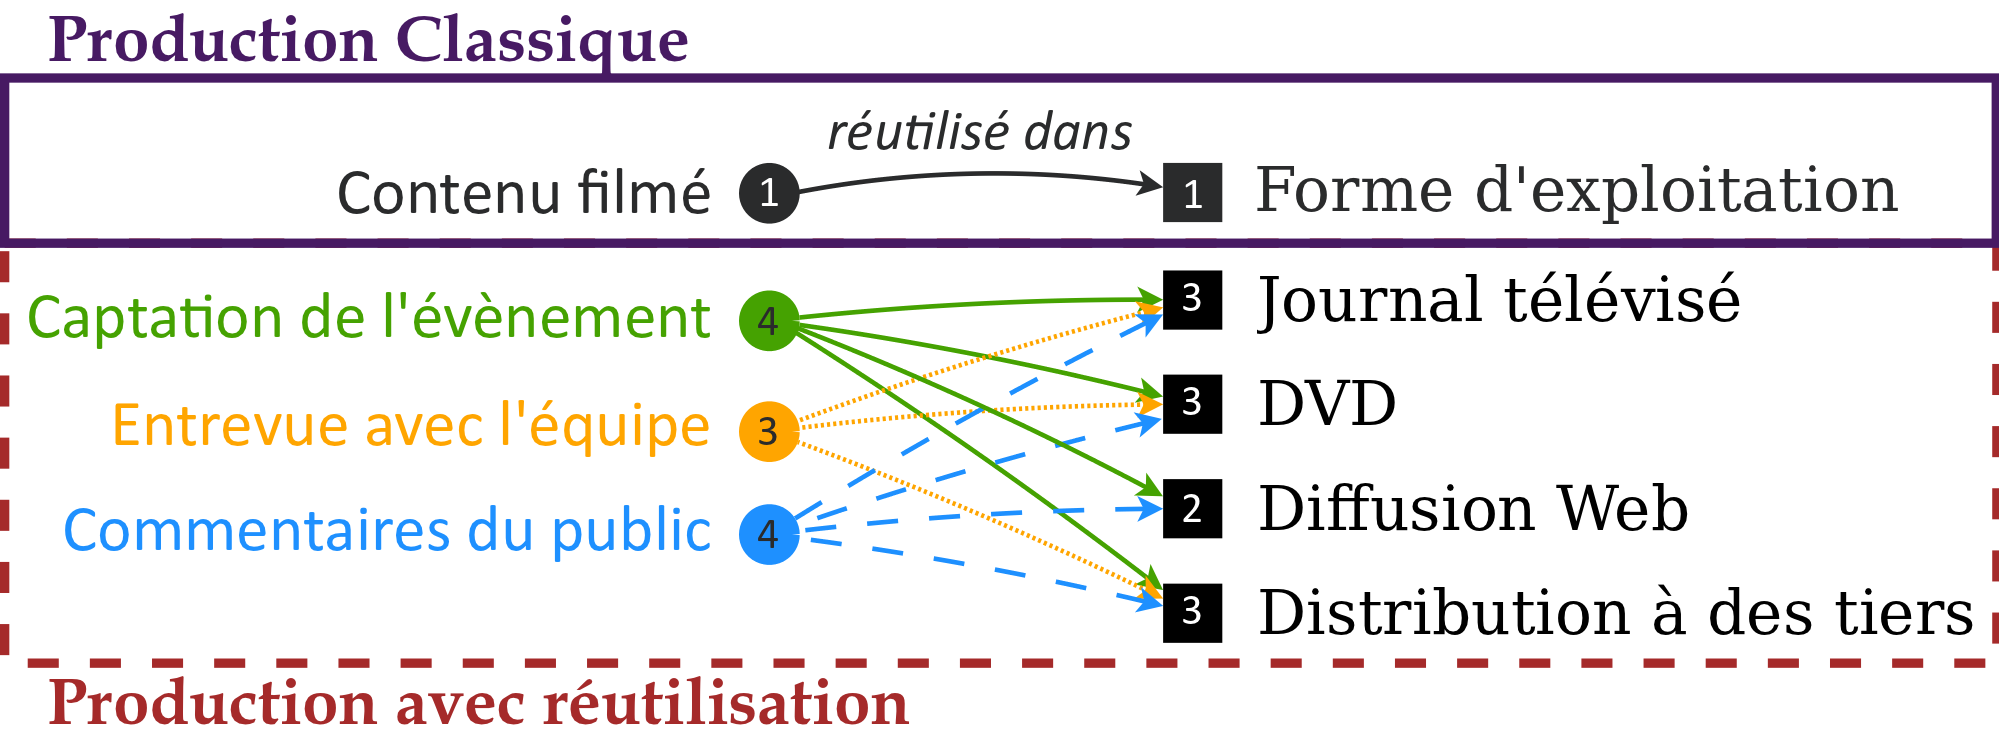
\includegraphics[width=0.7\textwidth]{images/UC-Tahnhauser-v1fr.png}
\caption{Modèle de la production classique comparé avec une production avec réutilisation}
\label{img:reuse}
\end{figure}


Chaque cas de réutilisation tire sa matière première d'à peu près la même base de contenu filmé, mais en tire partie d'une manière propre à chaque forme d'exploitation visée. 
En effet, chaque audience a ses attentes, de même qu'il existe des contraintes techniques spécifiques pour chaque contexte d'exploitation. 
%En effet, il existe des contraintes techniques et des attentes spécifiques à chaque contexte d'exploitation. 

Ces spécificités exigent des variations dans la qualité de l'encodage, le format d'encapsulation utilisé, le montage réalisé, l'habillage du contenu etc. 
Par exemple, les contraintes de diffusion sur le Web implique d'encoder la vidéo dans un format spécifique et de multiples résolutions, généralement plus petites que pour la diffusion télévisée. 
Ensuite, le montage d'une bande-annonce possède un rythme généralement plus rapide que celui des bonus de DVD. 
Finalement, les cas d'exploitation gérés par la chaîne de télévision posséderont un habillage spécifique (logo de la chaîne, message d'annonces etc.) que ne partageront pas forcément les versions vendues à des organisations tierces. 

L'exemple des commentaires du public -- voir la Figure \ref{img:intro:reuse-process} -- permet de montrer à quels moments des transformations doivent être effectuées afin de produire les différentes formes d'exploitation :
\begin{liste} 
	\item[$\bullet$] On considère que deux commentaires de spectateur ont été tournés. 
	\item[$\bullet$] Un des commentaires est intégré au montage du journal télévisé, alors que les deux sont utilisés pour créer la bande-annonce. La bande-annonce est elle-même intégrée au montage du DVD. 
	\item[$\bullet$] Au moment de la finition, l'encodage de la bande-annonce est adapté à la qualité DVD et Web. De même, le journal télévisé est encodé à la fois pour une diffusion en définition standard (SD) et haute-définition (HD).
\end{liste}


\begin{figure}[ht!]
\centering
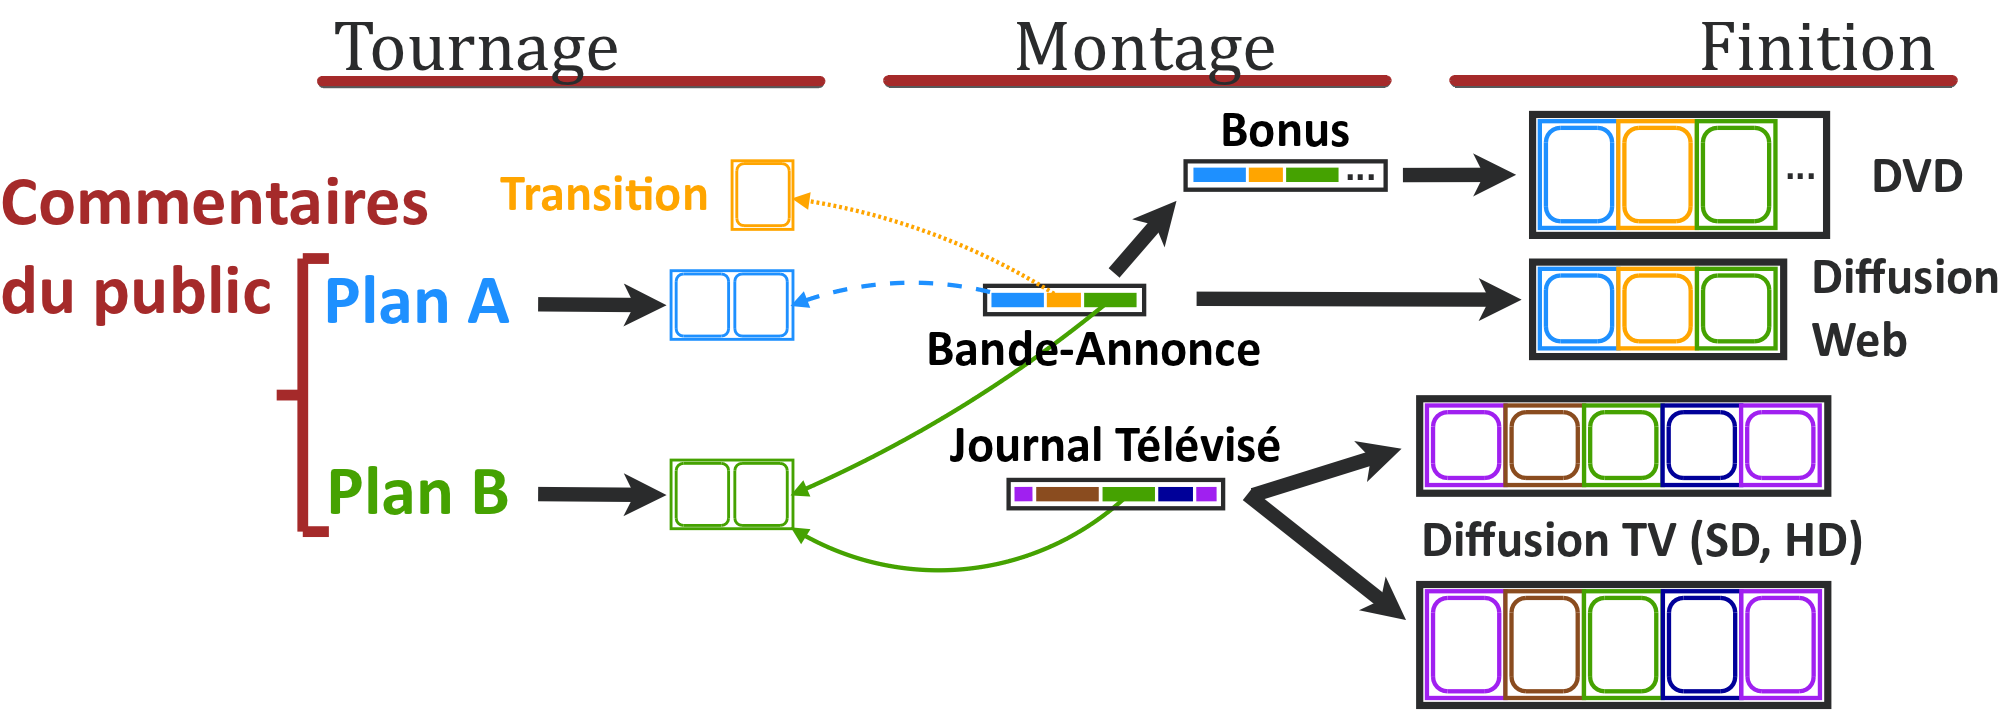
\includegraphics[width=0.8\textwidth]{images/EX-Content-Production-v7fr.png}
\caption{Étapes et transformations des contenus pour chaque forme d'exploitation des commentaires des spectateurs}
\label{img:intro:reuse-process}
\end{figure}

% Dans cet exemple, on distingue deux types d'opérations effectuées sur le contenu ; 
% la sélection de séquences au moment du montage qui correspond à une décision éditoriale (quel contenu va-t-on présenter à l'audience ?) ; 
% la tranformation de l'enregistrement du contenu qui correspond à des choix techniques (quelle méthode d'enregistrement va-t-on utiliser ?).
% Afin de préciser la nature de ces opérations, nous présentons différentes approches de la réutilisation des contenus.


\subsection{Besoins en modélisation}\label{sec:bm-av}
Le scénario d'usage que nous venons de voir présente un exemple de production incluant directement plusieurs formes d'exploitations pour des contenus produits en collaboration avec deux organisations professionelles et des amateurs. 
Ce scénario permet d'illustrer des opérations de transformation des contenus qui ne se limitent pas à une réutilisation brut de matériel vidéo. 
On distingue ainsi plusieurs types de transformations qui définissent nos besoins de modélisations :
\begin{liste}
	\item le \e{transcodage} d'un contenu d'un format/encodage/résolution à l'autre afin de satisfaire aux contraintes techniques propre à un medium ou un canal de distribution. 
	Par exemple, le journal télévisé distribué dans 2 types de définitions (SD, HD) ou bien la bande-annonce préparé pour une diffusion Web et DVD.
	%retraitement

	\item le \e{montage} différencié d'une séquence de contenu suivant la forme éditoriale dans laquelle elle s'insère.
	Le montage des commentaires du public est plus rapide et dense pour la bande-annonce que pour le journal télévisé. 
	Ce dernier prend plus de temps pour montrer les commentaires les plus construits ou les plus marquants.
	%rééditorialisation 

	\item l'\e{intégration} d'une séquence montée dans de multiple formes d'exploitations. 
	Par exemple, la bande-annonce est un montage de plusieurs commentaires du public. 
	Elle sert, telle quelle, à la fois sur le site Web de la chaîne et dans les bonus du DVD. 
\end{liste}

De plus, si l'on reprend le scénario depuis la commande de tournage, on se rend compte qu'il existe de nombreux types d'informations que l'on peut collecter sur les objets audiovisuels construits :
\begin{liste}
	\item le genre de l'objet audiovisuel à construire qui détermine un schéma de \e{structure éditoriale}. 
	\item la commande de tournage qui fait office de \e{prescription} de la forme et du contenu de l'objet à produire.
	\item le tournage dont le résultat constitue la \e{réalisation} de la commande, c'est-à-dire le fichier vidéo créé.
	\item une fois le contenu produit, on peut en établir une \e{description} qui se révèlera plus ou moins proche de la prescription.
	\item le montage qui détermine la \e{composition} de l'objet audiovisuel.
	\item l'\e{organisation de la production} de manière générale, c'est-à-dire la division des tâches entre contributeurs. 
\end{liste}

Nos besoins en modélisations peuvent donc se résumer par les assertions suivantes : 
\begin{liste}
	\item[(\e{B1}]\e{ : autonomie}) rendre les objets et les fragments audiovisuels autonomes implique de les modéliser sur différents niveaux (technique, esthétique, éditorial etc.). 
	Chaque niveau de modélisation correspond au résultat d'opérations effectuées durant le processus de production audiovisuel.
	Ainsi, chaque niveau peut être pris séparément de l'ensemble.
	%(\g{B1 : autonomie})

	\item[(\e{B2}]\e{ : réutilisabilité}) rendre les objets et les fragments audiovisuels réutilisables implique de leur associer de multiples connaissances dès le début et tout au long de leur cycle de vie.
	Ces connaissances doivent correspondre à celles mobilisées par les contributeurs (humain ou logiciel) de la chaîne de production.
	Chaque type de connaissance s'associe à un niveau spécifique de l'objet audiovisuel pour le décrire et ainsi faciliter sa recherche.
	%(\g{B2 : réutilisabilité})
	% \item[(B3)] : 
\end{liste}

% À chaque niveau de modélisation des objets et fragments audiovisuels correspond des types de connaissances. 
On notera que la modélisation des objets et des connaissances associées vont de pair et suivent le déroulement de la chaîne de production.
Ainsi, ce n'est plus seulement le résultat final de la production qui est modélisé, mais l'ensemble du processus.
Chaque résultat est modélisé séparément, relié à l'ensemble et décrit par des connaissances récoltées pendant sa construction, ce qui confère à la modélisation ces propriétés d'autonomie et de réutilisabilité.
Cette finesse de modélisation ne peut s'obtenir qu'à partir d'une compréhension plus complète de la chaîne et donc plus centrée sur les métiers de la production audiovisuelle. 